% !Mode:: "TeX:UTF-8"
\chapter{引言}
\label{ch:intro}
本章主要介绍了自动驾驶的技术背景以及三维物体检测在自动驾驶技术中的重要作用,然后引出了目前三维物体检测技术的局限性。之后,本章介绍了目前国内外对三维物体检测的研究进展,也简单介绍了三维多目标追踪的研究进展。最后,本章简要概括了本文的工作重点以及技术创新要点,强调了本文研究对于自动驾驶领域的重要意义。

\section{研究背景与意义}
\label{sec:background}
近几年来, 深度学习的迅猛发展赋予了机器越来越强的智能。在计算机视觉、自然语言处理等领域的某些任务上,机器甚至能够表现出比人类更好的性能\cite{he2016deep,DevlinBERT}。 在这样的大背景下, 无人驾驶(Autonomous Driving) 作为最能够体现机器智能的应用场景之一,受到了学术界和工业界的广泛关注。 无人驾驶要求机器能够像人类一样识别道路场景,包括行人和车辆的状态以及车道线等,并且能够根据这些信息高效地进行路径规划来实现与人类类似的驾驶行为。 无人驾驶应用十分广泛,无论是民用还是军工领域。 机器取代人类驾驶车辆,一方面能让人们出行效率更高, 另一方面,机器之间的通讯比人类效率更高,这使得车辆能够更好的规划自己的行驶路径,降低交通事故发生概率。作为智慧城市的不可缺少的组成部分, 无人驾驶也能在非常时期发挥重要作用。譬如在面对重大传染病时(如2019年末爆发的COVID-19),人员之间要尽量减少接触,此时无人驾驶能在保证安全的情况下,极大方便人们的日常生活,包括出行以及货物配送。因此,无人驾驶作为可预见的未来技术,一直是各国在高科技领域的“必争之地”。近十几年来,国内外的无人驾驶平台如雨后春笋般冒出,既有老牌互联网大公司开展的新业务,如国内百度的Apollo\footnote[1]{http://apollo.auto/}(如\figurename \ref{fig:apollo}),美国Google的Waymo\footnote[2]{https://waymo.com/}(如\figurename \ref{fig:waymo})等;也有新型汽车行业巨头,如Uber、特斯拉、滴滴、上汽等;另外,还有新兴的无人驾驶创业公司,如pony.ai、图森未来、驭势科技等。这些都是推动无人驾驶商业化不可忽视的力量,也是推动无人驾驶技术落地的中坚力量。

\begin{figure}[!t]
	\centering
	\begin{minipage}[t]{0.40\textwidth}
		\centering
		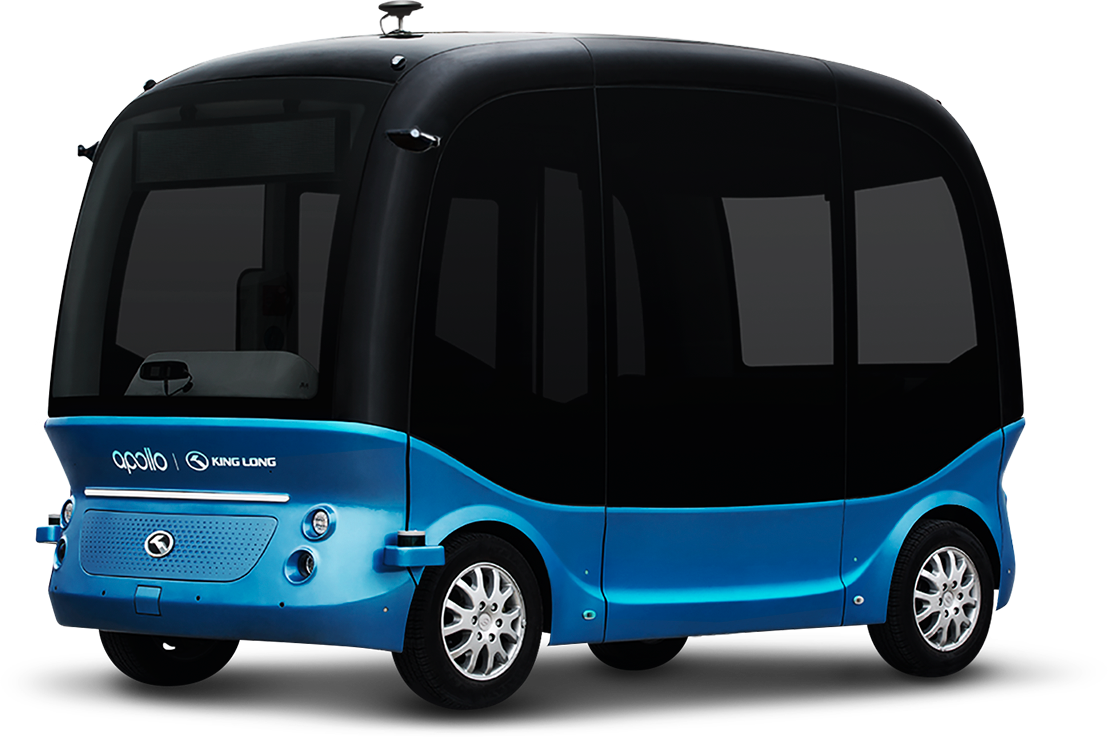
\includegraphics[width=\textwidth]{./imgs/apollo.png}
		\caption{Apollo自动驾驶汽车}
		\label{fig:apollo}
	\end{minipage}
	\begin{minipage}[t]{0.55\textwidth}
		\centering
		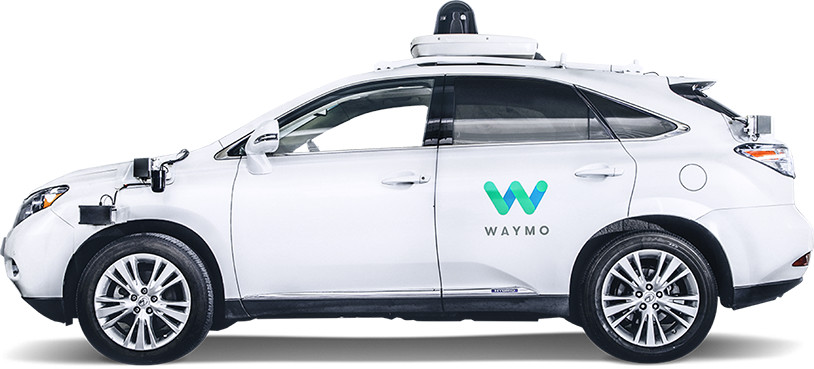
\includegraphics[width=\textwidth]{./imgs/waymo.jpg}
		\caption{Waymo自动驾驶汽车}
		\label{fig:waymo}
	\end{minipage}
\end{figure}


无人驾驶技术主要包括感知、决策和规划三个重要模块,其中感知模块是无人驾驶技术的基础,也是难点。感知模块的任务是赋予机器理解环境的能力,使机器能够准确捕获复杂道路场景的有用信息。目前无人驾驶车辆依赖多种传感器感知环境, 譬如激光雷达(LIDAR)、摄像头、毫米波雷达等。这些传感器都有着各自的优缺点,特别是在价格、使用场景以及探测距离方面,如表\ref{table:sensor_cmp}所示。因此,目前绝大多数自动驾驶公司在感知模块都使用多传感器融合技术,让各传感器优劣互补。多传感器采集的数据会通过算法进行融合,尽可能准确的还原真实的三维环境信息,以便用于后续的目标检测以及跟踪等任务。

\begin{table}
	\centering
	\wuhao
	\caption{自动驾驶各传感器对比\cite{FirstAVbook}。}
	\vspace{0.3cm}
	\resizebox{\textwidth}{!}{
		\begin{tabular}{cccccccc}
			\toprule[1.5pt]
			传感器    & 激光雷达(LIDAR) & 摄像头(Camera) & 毫米波雷达 \\ \midrule
			外形      & \begin{minipage}{0.13\textwidth}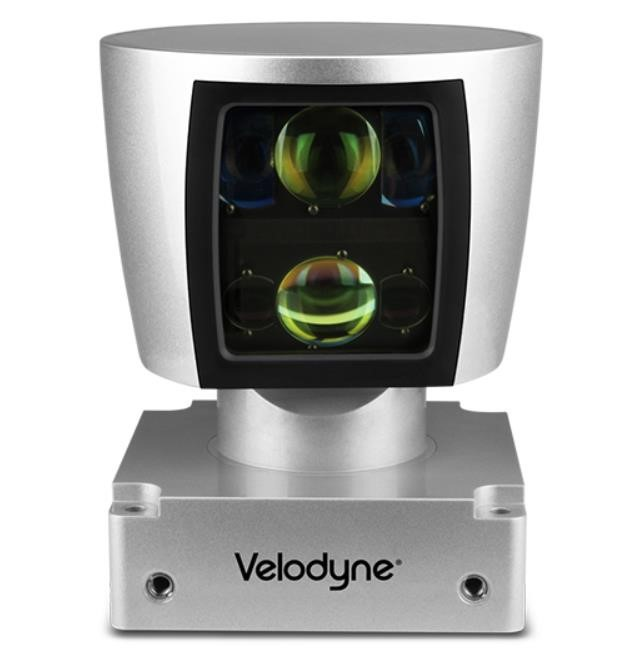
\includegraphics[width=\linewidth]{../figures/imgs/lidar.jpg}\end{minipage} & \begin{minipage}{0.15\textwidth}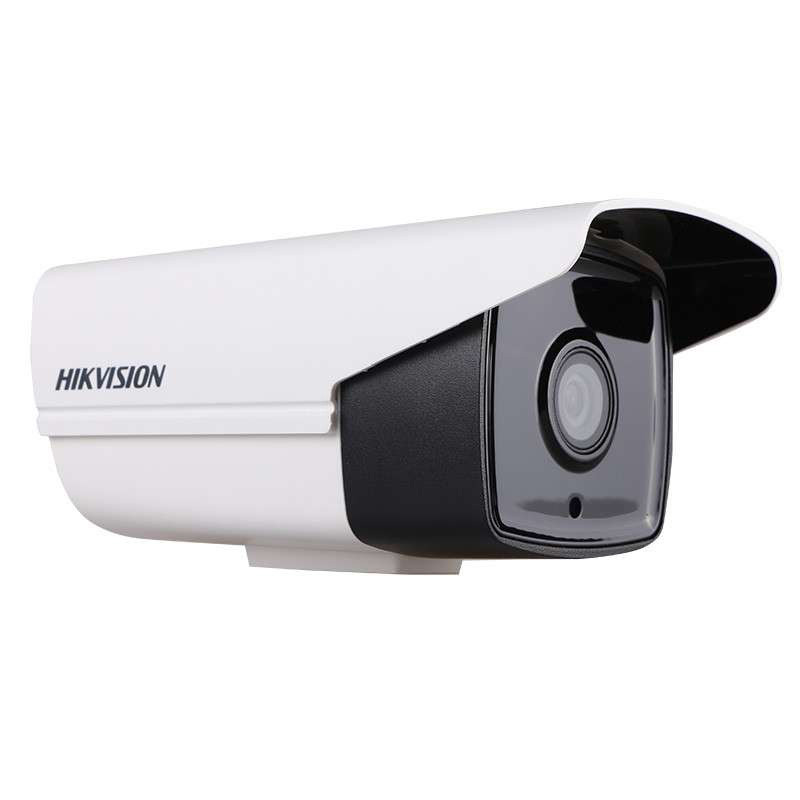
\includegraphics[width=\linewidth]{../figures/imgs/camera.jpg}\end{minipage} & \begin{minipage}{0.15\textwidth}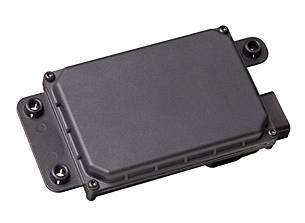
\includegraphics[width=\linewidth]{../figures/imgs/mlidar.jpeg}\end{minipage} \\ \hline
			价格      & 8000美元以上    & 35-50美元         & 300-500美元    \\ \hline
			优点      & \makecell*[c]{扫描周围环境得到精确\\环境信息、距离信息}   & \makecell*[c]{成本比较低,通过算法\\可以实现各种功能} & \makecell*[c]{不受天气影响,\\测量精度高}  \\ \hline
			缺点      & \makecell*[c]{成本高,大雾、雨雪天气\\效果差,无法图像识别}  & \makecell*[c]{恶劣环境下失效,难以测距,\\探测距离较近,算法要求高}   & \makecell*[c]{无法识别道路指示牌,\\无法识别行人}   \\ 
			\bottomrule[1.5pt]
	\end{tabular}}
	\label{table:sensor_cmp}
\end{table}


环境感知中一大核心任务是物体检测(Object Detection), 即通过分析传感器采集的数据,确定环境中各目标的位姿,包括其在世界坐标系下的坐标、形状信息以及朝向。不同于以图像为主要数据载体的二维物体检测,自动驾驶领域的物体检测任务要求预测目标在三维空间的位姿信息,即三维目标检测。三维目标检测比二维目标检测更加具有挑战性,这是因为维度诅咒(the curse of dimensionality)的存在: 当维度增加时,空间的体积增加的非常之快(以指数增加),以致于可用的数据变得稀疏。 三维物体检测的一大挑战,就是三维数据的稀疏性。目前无人驾驶中三维数据的获得主要是依靠激光雷达,其原理是通过高速旋转的激光发射器向周围发射激光,然后检测接收到反射回来光线的时间间隔来计算反射点的距离。激光雷达的线束对其分辨率有很大影响,特别是对于远距离的目标,在低线束(例如16线)激光雷达中可能只有稀疏的几个点,完全无法分辨。而分辨率高的高线束的激光雷达则十分昂贵,以 Velodyne 64线激光雷达为例,其价格高达十几万美金,因此多数无人驾驶技术方案都需要在激光雷达分辨率与价格之间做出权衡。最近一种非完全旋转的激光雷达——固态激光雷达\footnote[3]{http://www.robosense.cn/rslidar/rs-lidar-m1}受到越来越多人的关注,它们具备数据采集速度快、分辨率高、价格低廉以及环境适应性强等特点,被自动驾驶行业给予厚望。然而目前该技术尚不成熟,还没经过广泛的实际场景检验,离落地还有一段时间,因此暂时不在各大方案的候选传感器之内。短期来看,传统的机械式激光雷达仍是各大自动驾驶平台的首选。

根据使用传感器数据的不同,目前三维物体检测的研究主要有三个方向:基于图像数据的方案\cite{7780605, chen20183d},基于点云数据的方案\cite{li20173d,engelcke2017vote3deep,zhou2018voxelnet,simon2018complex,shi2019pointrcnn},以及基于多传感器数据融合的方案\cite{qi2018frustum,chen2017multi,ku2018joint}。借助深度学习技术,这些方案都取得了很不错的结果。尽管如此,目前基本所有的三维物体检测方案都是针对单帧数据进行检测。对于真实的自动驾驶场景的物体检测任务来说,数据都是以流的形式连续获取的。从算法落地的难易程度方面考虑,开发针对流数据的三维物体检测算法相比于基于单帧的三维物体检查算法更加具有优势。相比于单帧数据,流数据可以提供同一目标在一段时间内的连续信息。一方面,由于检测噪声(误检测的物体)在时间维度上连续性较差,因此时序上的连续信息有利于检测算法筛除误检测的目标。另一方面,对于遮挡以及物体框被边界截断的目标,在流数据中可以利用前后帧的信息对其进行补全,从而获得更好的检测性能,这对于基于单帧的检测算法来说是难以实现的。最后值得注意的是,流数据一般有很强的数据冗余性,即相邻帧之间绝大多数信息都相同,只有存在物体运动的区域才会有些许差异。对于流数据物体检测,如果使用基于单帧的物体检测算法,则需要逐帧进行检测,然后再将结果关联,这个过程会存在很多重复计算的过程,十分耗时。但是如果使用基于流数据的物体检测算法,则有可能只对少量帧(例如关键帧)进行检测,然后利用流数据的冗余性与时序信息将检测结果传播到其余帧,从而能够更为高效的完成三维物体检测任务。 因此,将基于单帧的三维物体检测算法扩展到流数据场景,能显著提高三维物体检测算法的准确率与效率,也是将三维物体检测技术落实到实际场景的必经之路,具有很强的实践意义。本工作旨在探索基于关键帧的三维流数据物体检测框架,同时也探究了三维时序信息的特征编码以及预测框的传播算法,为后续三维目标检测算法的落地工作提供一个可行的参考方案。

\section{国内外研究进展}
\label{sec:realted_work}
目前国内外针对流数据的三维物体检测研究还较少,而基于单帧数据的三维物体检测以及基于视频流的二维物体检测的研究较为丰富。 因此,本节分别从三维物体检测以及视频流物体检测概述前沿进展。 另外,三维场景的多目标追踪研究进展也会进行简要说明。

\subsection{三维物体检测}
\label{3d_detect}
目前大多数三维检测研究可以归类为三大方向:基于图像,基于点云,以及基于多传感器融合。 

(1)基于图像的方法。 基于图像的三维物体检测以 Mono3D \cite{7780605} 和 3DOP \cite{chen20183d} 为代表。 这类方法只是用摄像头采集的图像数据,通过多视角图像融合来推断三维信息。由于图像数据没有深度信息,这类方法需要人工设计的几何特征来表征物体的深度信息,虽然数据采集简单,速度快,但是检测精度差。 最近越来越多研究者探索基于双目摄像头数据的三维物体检测,例如 [TODO]。 这类方法通过神经网络融合左右摄像头的数据来预测物体的三维信息, 从生物学上来说很接近人类的双眼视觉系统。 然而由于神经网络的不确定性,以及双目视觉盲区的存在,该方法仍然有很多亟待解决的问题。

(2)基于点云的方法。 基于点云的方法可分为一步法和两步法。 一步法即直接是端对端预测物体的三维位姿,这类方法根据点云的编码方式不同又可分为基于体素的方法以及基于投影的方法。 基于体素的方法使用三维体素网格编码点云特征, 每个体素立方体的值由该立方体内的点决定,从而将不规则的三维点云数据编码成规则的三维体素数据, 便于后续使用神经网络进行特征提取。 代表有 3D FCN \cite{li20173d}, Vote3Deep \cite{engelcke2017vote3deep}以及 VoxelNet \cite{zhou2018voxelnet}等。 这类方法的一大缺点是体素大小不好确定,太大的话信息损失严重,太小则会造成巨大的计算量。 另外,这类方法需要使用到三维卷积,因此很耗计算资源。 基于投影的方法是将点云在高度方向进行投影,将三维数据降维成二维的俯视图(BEV, bird eye view)数据。 考虑到驾驶场景中, 道路基本是共面且水平的,因此在高度方向上投影对物体的位姿信息基本没有损失。 经过投影操作后,就能直接使用二维图像物体检测的方法进行物体检测。 PIXOR \cite{yang2018pixor} 以及 Complex-YOLO \cite{simon2018complex,Simon_2019_CVPR_Workshops} 等属于这类方法。 虽然降维能够带来速度的极大提升,然而由于点云数据的稀疏性,经过投影后目标的特征点损失很严重。 特征点的不足会很大程度上影响检测结果的准确性,特别是对于远处的目标以及小目标。 两步法的思路是先对点云进行分割, 然后对于分割结果的每一个目标进行框回归,得到目标的三维位姿信息。 这类方法的代表有 \cite{shi2019pointrcnn}。 两步法的不足之处是其检测结果非常依赖于分割结果,且在框回归中,对于点较少的远处目标,三维位姿信息的恢复效果并不好。

(3)基于多传感器融合的方法。 点云的稀疏性以及图像缺少深度信息都限制着相应方法的准确率,一个自然而然的想法就是能不能将这两种数据融合, 从而达到更好的检测结果。 基于多传感器融合的方法通过算法融合点云数据以及图像数据,从而提升三维物体检测的准确率。 这类方法的代表有 F-PointNet \cite{qi2018frustum}, MV3D \cite{chen2017multi}, AVOD \cite{ku2018joint}等。 这些方法的区别主要在于融合的方式不同, F-PointNet 首先使用二维物体检测方法检测出图像中的所有物体,之后对于每个物体,将其反投影回点云中得到一个视锥区域,对该区域内的点进行分割然后再进行框回归。该方法通过先在图像中找出目标,从而减少了在点云空间的搜索区域。然而,该算法的准确率受二维物体检测很大,在第一步没有检测出的物体,之后没有其他办法弥补。 MV3D 将二维物体检测中的的区域提取网络 (Region Proposal Network, RPN) 扩展到三维, 提出了 3D RPN 分别提取点云以及图像特征, 然后通过一个特征融合模块得到融合特征,最后进行三维物体检测。 AVOD 在 MV3D 的基础上改进了特征提取模块, 引入的金字塔结构从而能够得到全分辨率的特征图, 提升了物体的定位精度,特别对于小物体。 本文工作基于 AVOD 框架并进行了改进, 使其能支持多针输入, 并且引入了时序信息处理模块。

\subsection{视频流物体检测}
\label{video_detect}
视频流物体检测与单帧物体检测的主要区别在于是否利用了时序信息。 对于视频流物体检测,时序信息是物体的位姿在时间上的连续性的抽象体现。 目前,大多数视频流物体检测方法都是在两个层面利用时序信息,特征提取层面以及最终的框回归层面。 对于特征处理层面, 一般是根据运动信息将前后帧的的特征整合到关键帧,以增加关键帧的物体特征。 这个过程中需要使用到光流信息,即图像中各像素点的运动方向。 代表有 FGFA \cite{zhu2017flow}系列工作。 一般来说光流信息的获取比较困难,这也是限制该方法进一步发展的主要障碍。 对于在框回归层面利用时序信息,主要的工作有 T-CNN \cite{kang2018t, kang2016object} 与 Seq-NMS \cite{han2016seq}等。 T-CNN 使用预先计算的光流信息将关键帧的检测结果传播到临近帧,而 Seq-NMS 则是通过整合连续几帧的高置信度的候选框来提升目标检测中非极大值抑制(Non-Maximum Suppression,NMS)算法的性能。 最近, 也有一些工作试图通过神经网络学习连续帧之间的的时序信息, 从而避免使用高代价的光流数据。 这类方法的代表有 D\&T \cite{feichtenhofer2017detect}。 D\&T 提出了一个双路目标检测网络,可以同时时间视频流的目标检测以及目标追踪。 该网络可以输入多帧数据进行检测, 并且通过互相关操作(Cross-correlation) 来学习相邻帧之间相同物体的对应关系以及偏移。 本文的算法框架在一定程度上也借鉴了 D\&T 的结构, 不过我们在他的基础上进行了很大的改进,使其能够适应三维物体的流数据检测。

\subsection{三维多目标追踪}
\label{tracking}
目前基本上所有的三维多目标追踪方法都是先对流数据的每一帧进行目标检测,然后再将这些检测框关联起来, 这种范式也被称为 \textit{Tracking by Detection} \cite{lenz2015followme}。 三维多目标追踪的工作有很多,比较有代表性的有 FaF \cite{luo2018fast}, 3D-CNN/PMBM \cite{scheidegger2018mono}以及 DSM \cite{frossard2018end}等。 FaF 使用首先将点云流数据结构化成四维张量,然后构建了一个简单的特征提取网络提取特征,最后使用不同的网络头分别预测得到三维目标检测,多目标追踪以及运动方向预测结果。该方法能够整合前 $n$ 帧的检测结果得到精确的物体运动轨迹。 然而该方法计算量巨大, 并且网络参数调节需要有很高的技巧。  3D-CNN/PMBM 首先构建神经网络从单张图像预测物体的三维位姿, 然后将所有帧的检测框送入泊松多重伯努利 (Poisson Multi-Bernoulli Mixture, PMBM) 混合追踪滤波器进行滤波,得到最终的三维多目标追踪结果。 该方法只使用单帧图像进行三维目标检测,效果有限。 DSM 首先使用单帧三维物体检测框架 MV3D \cite{chen2017multi} 对每一帧数据进行物体检测得到三维检测框, 然后通过一个匹配网络(\textit{Matching net})以及得分网络(\textit{Scoring net})关联所有的检测框。 该方法需要对每一帧数据都进行检测, 并且帧与帧之间的时序信息基本上没有被使用,因此不是针对流数据的高效方法。

\section{本文工作及创新点}
\label{subsec:contribution}
本文提出了一个双路物体检测与追踪(\textbf{D}ual-way \textbf{O}bject \textbf{D}etection and \textbf{T}racking, \textbf{DODT})框架, 实现了流数据场景的高效三维物体检测与追踪。 本框架的构建是基于以下几个观察: (1) 点云能够与图像融合从而丰富物体的视觉特征, 这点在 \cite{chen2017multi,ku2018joint}中得到了证实; (2) 除了通过光流数据, 时序信息也能够通过计算相邻帧间的互相关信息,这点通过 \cite{feichtenhofer2017detect} 也能够得到验证; (3) 特征在连续帧之间的变化是连续的, 我们可以只对关键帧进行检测,然后将结果传播到非关键帧, 这样可以极大的减少计算量。 对于第一点, 本文借用了 AVOD\cite{ku2018joint} 中的数据融合方案,将点云数据提供的 BEV 信息与图像融合。 对于第二点, 本文构建了一个时序模块(Temporal module), 该模块使用互相光操作在 BEV 空间中计算相邻关键帧的时序特征, 然后预测相同物体在不同关键帧中同时出现的概率以及偏移量。 与 \cite{feichtenhofer2017detect,dosovitskiy2015flownet} 不同的是, 本模块的互相关操作是在后候选框层面进行的,不需要全局计算, 这极大地提高了模块的运行效率。 对于最后一点, 我们将 DODT 框架的目标检测模块设计成了双路结构, 这样该模块就能够同时输入两帧相邻关键帧, 以保证后面时序模块的正确运行。 另外, 为了进一步提高框架的效率, 本文还设计了一个共享 RPN (Shared Region Proposal Network, Shared RPN) 模块, 该模块可以生成供两检测分支共同使用的三维候选框。 最后,为了生成所有帧的检测结果, 本文设计了一个基于运动的框插值算法, 该算法利用关键帧的检测结果以及时序模块预测的信息,插值生成非关键帧的检测结果。 同时, 该差值算法还能够将不同帧的候选框关联起来, 得到多目标追踪结果。

本文的贡献及创新点如下:
\begin{itemize}
	\item 本文提出了名为 DODT 的双路网络, 该网络能够同时精确地完成基于流数据的三维物体检测以及多目标追踪任务。
	\item 本文提出了一个时序模块在候选框层面上编码相邻关键帧之间的时序信息, 相比于\cite{feichtenhofer2017detect,dosovitskiy2015flownet}中方法, 该方法更加灵活,也更加高效。
	\item 本文设计了一个共享 RPN 模块, 能够显著提高相邻多帧目标检测中候选框提取的效率。
	\item 本文开发了一个基于运动的框插值算法, 能够有效的将关键帧的预测框传播到非关键帧, 同时也能够将所有框关联起来, 实现多目标追踪。
\end{itemize}


\section{文章组织与结构}
\label{subsec:structure}
本文的主要内容分为五章。 第一章为引言, 介绍项目的研究背景和意义, 国内外的研究进展以及本文工作的简单介绍和创新点; 第二章介绍本工作涉及到的一些技术的基础理论, 分为目标检测与目标追踪两大块; 第三章详细地介绍了本文提出的框架的构造和原理, 是全文的重点内容; 第四章主要是介绍了本项目的实验设计, 结果展示以及实验结果分析, 该部分也是全文的重点内容; 最后一章总结本文的工作, 然后介绍本文工作的不足之处以及后续的实验计划。 


% 打印时插入必要的空白页
\ifprint
	\newpage
	\thispagestyle{empty}
	\mbox{}
	
	% 避免空白页影响页码编号
	\clearpage
	\setcounter{page}{10}
\fi